\documentclass[11pt]{article}
\usepackage[margin=1in]{geometry}
\usepackage{xcolor}
\usepackage[breakable]{tcolorbox}
\usepackage{hyperref}
\usepackage{enumitem}
\usepackage{listings}
\usepackage{verbatim}
\usepackage{amsmath}
\usepackage{graphicx}
\usepackage{booktabs}
\usepackage{float}

% Define colors
\definecolor{osaorange}{RGB}{220,115,38}
\definecolor{codebackground}{RGB}{248,248,248}

% Configure hyperref
\hypersetup{
    colorlinks=true,
    linkcolor=blue,
    urlcolor=blue,
    citecolor=blue
}

% Simple framed code environment
\usepackage{fancyvrb}
\DefineVerbatimEnvironment{rcode}{Verbatim}{
  fontsize=\small,
  frame=single,
  framesep=3pt,
  rulecolor=\color{gray!50}
}

% This approach uses tcolorbox with automatic line breaking and proper margins

\title{}
\author{}
\date{}

\begin{document}

% Header box
\begin{tcolorbox}[colback=osaorange,colframe=black,boxrule=2pt,arc=0pt,left=3pt,right=3pt,top=6pt,bottom=6pt,boxsep=2pt]
\centering
\textcolor{white}{\textbf{\Large H524 Introduction to Biostatistics}}\\
\textcolor{white}{\textbf{\Large Week 1 Lab: Introduction to R and Data Visualization}}\\
\textcolor{white}{\textbf{\Large Fall 2025}}
\end{tcolorbox}

\vspace{8pt}

\noindent\textbf{Lab Duration:} 110 minutes (8:00am -- 9:50am)\\
\textbf{Format:} Online\\
\textbf{Tools Required:} R, RStudio

\section{Learning Objectives}

By the end of this lab, you will be able to:
\begin{enumerate}
\item Set up R and RStudio for biostatistical analysis
\item Create and manipulate basic R data structures
\item Generate descriptive statistics for health data
\item Create publication-quality visualizations for different data types
\end{enumerate}

\section{Lab Setup}

\subsection{Required Software}
\begin{enumerate}
\item \textbf{R:} Download from \url{https://cran.r-project.org/}
\item \textbf{RStudio:} Download from \url{https://posit.co/products/open-source/rstudio/}
\end{enumerate}

\subsection{Verify Installation}
Open RStudio and run the following code to verify your setup:

\begin{rcode}
# Check R version
R.version.string

# Check working directory
getwd()

# Test basic functionality
x <- c(1, 2, 3, 4, 5)
mean(x)
\end{rcode}

\section{Part 1: R Fundamentals (30 minutes)}

\subsection{Data Types and Structures}

\textbf{Exercise 1.1:} Create variables of different data types relevant to health research.

\textbf{Note:} The health data used in these exercises are simulated values designed for demonstration purposes. They represent typical ranges found in clinical practice but are not from actual patient records.

\begin{rcode}
# Numeric data (simulated systolic/diastolic blood pressure values)
systolic_bp <- c(120, 135, 142, 118, 160, 125, 138)
diastolic_bp <- c(80, 85, 92, 75, 95, 82, 88)

# Character data
patient_id <- c("P001", "P002", "P003", "P004", "P005", "P006", "P007")
gender <- c("Male", "Female", "Female", "Male", "Male", "Female", "Male")

# Factor data (categorical)
treatment_group <- factor(c("Control", "Treatment", "Treatment",
                           "Control", "Treatment", "Control", "Treatment"))

# Logical data
hypertensive <- systolic_bp >= 140 | diastolic_bp >= 90

# Display the data types
class(systolic_bp)
class(gender)
class(treatment_group)
class(hypertensive)
\end{rcode}

\textbf{Exercise 1.2:} Create a data frame combining health variables.

\begin{rcode}
# Create a comprehensive health dataset (based on 2024 materials)
health_data <- data.frame(
  patient_id = patient_id,
  gender = gender,
  systolic_bp = systolic_bp,
  diastolic_bp = diastolic_bp,
  treatment_group = treatment_group,
  hypertensive = hypertensive,
  age = c(45, 52, 38, 61, 47, 34, 55),
  weight_kg = c(75, 68, 82, 71, 88, 63, 79),
  height_cm = c(170, 165, 178, 172, 180, 160, 175)
)

# View the data structure
str(health_data)
head(health_data)
summary(health_data)
\end{rcode}

\section{Part 2: Descriptive Statistics (25 minutes)}

\textbf{Exercise 2.1:} Calculate measures of central tendency and variability.

\begin{rcode}
# Measures of central tendency
mean_systolic <- mean(health_data$systolic_bp)
median_systolic <- median(health_data$systolic_bp)

# Measures of variability
sd_systolic <- sd(health_data$systolic_bp)
var_systolic <- var(health_data$systolic_bp)
range_systolic <- range(health_data$systolic_bp)
iqr_systolic <- IQR(health_data$systolic_bp)

# Display results
cat("Mean systolic BP:", round(mean_systolic, 2), "mmHg\n")
cat("Median systolic BP:", median_systolic, "mmHg\n")
cat("Standard deviation:", round(sd_systolic, 2), "mmHg\n")
cat("Range:", range_systolic[1], "-", range_systolic[2], "mmHg\n")
\end{rcode}

\textbf{Exercise 2.2:} Generate descriptive statistics by group.

\begin{rcode}
# Statistics by gender
aggregate(systolic_bp ~ gender, data = health_data, FUN = mean)
aggregate(systolic_bp ~ gender, data = health_data, FUN = sd)

# Statistics by treatment group
aggregate(systolic_bp ~ treatment_group, data = health_data, FUN = summary)

# Frequency tables for categorical data
table(health_data$gender)
table(health_data$treatment_group)
prop.table(table(health_data$hypertensive))
\end{rcode}

\section{Part 3: Data Visualization (35 minutes)}

\subsection{Geographic Health Mapping}

\textbf{Exercise 3.1:} Create health-focused maps (mirroring 2024 approach).

\begin{rcode}
# Install required packages for mapping (if not already installed)
# install.packages(c("maps", "mapdata", "ggplot2"))
library(maps)
library(mapdata)
library(ggplot2)

# Create simulated state-level health data
state_health <- data.frame(
  state = c("oregon", "washington", "california", "nevada", "idaho"),
  diabetes_rate = c(8.2, 9.1, 9.7, 10.8, 8.9),
  obesity_rate = c(28.7, 27.9, 25.1, 26.8, 29.2)
)

# Get US state map data
states_map <- map_data("state")

# Merge health data with map coordinates
map_data <- merge(states_map, state_health, by.x = "region", by.y = "state")

# Create diabetes prevalence map
ggplot(map_data, aes(x = long, y = lat, group = group, fill = diabetes_rate)) +
  geom_polygon(color = "white") +
  scale_fill_gradient(low = "lightblue", high = "darkred",
                      name = "Diabetes Rate (%)") +
  coord_quickmap() +
  theme_void() +
  labs(title = "Diabetes Prevalence by State",
       subtitle = "Simulated data for demonstration")
\end{rcode}

\begin{figure}[H]
\centering
\fbox{\parbox{0.8\textwidth}{
\textbf{Output:} This code will generate a choropleth map showing diabetes prevalence rates across Pacific Northwest states. Higher rates appear in darker red, with Washington and Nevada showing elevated diabetes prevalence compared to Oregon and California.
}}
\caption{Geographic visualization of diabetes prevalence rates (code output shown)}
\end{figure}

\subsection{Visualizations for Continuous Data}

\textbf{Exercise 3.2:} Create histograms and box plots with enhanced features.

\begin{rcode}
# Histogram of systolic blood pressure
hist(health_data$systolic_bp,
     main = "Distribution of Systolic Blood Pressure",
     xlab = "Systolic BP (mmHg)",
     ylab = "Frequency",
     col = "lightblue",
     border = "white",
     breaks = 5)

# Add vertical line for mean
abline(v = mean_systolic, col = "red", lwd = 2, lty = 2)
legend("topright", "Mean", col = "red", lwd = 2, lty = 2)

# Box plot by gender
boxplot(systolic_bp ~ gender,
        data = health_data,
        main = "Systolic BP by Gender",
        ylab = "Systolic BP (mmHg)",
        col = c("pink", "lightblue"))
\end{rcode}

\begin{figure}[H]
\centering
\fbox{\parbox{0.7\textwidth}{
\textbf{Output:} Histogram displays systolic blood pressure distribution with blue bars, white borders, and a red dashed vertical line indicating the mean value (approximately 135 mmHg).
}}
\caption{Example histogram showing blood pressure distribution with mean line}
\end{figure}

\begin{figure}[H]
\centering
\fbox{\parbox{0.7\textwidth}{
\textbf{Output:} Side-by-side box plots comparing systolic blood pressure between males (light blue) and females (pink), showing median, quartiles, and any outliers.
}}
\caption{Example box plot comparing blood pressure by gender}
\end{figure}

\subsection{Advanced Health Visualizations}

\textbf{Exercise 3.3:} Create BMI analysis with multiple plot types.

\begin{rcode}
# Calculate BMI and categorize
health_data$bmi <- health_data$weight_kg / (health_data$height_cm/100)^2
health_data$bmi_category <- cut(health_data$bmi,
                                breaks = c(0, 18.5, 25, 30, Inf),
                                labels = c("Underweight", "Normal", "Overweight", "Obese"))

# Create comprehensive BMI visualization
par(mfrow = c(2, 2))  # 2x2 plot layout

# 1. BMI histogram with normal curve overlay
hist(health_data$bmi, probability = TRUE,
     main = "BMI Distribution", xlab = "BMI", col = "lightblue")
curve(dnorm(x, mean = mean(health_data$bmi), sd = sd(health_data$bmi)),
      add = TRUE, col = "red", lwd = 2)

# 2. BMI by gender boxplot
boxplot(bmi ~ gender, data = health_data,
        main = "BMI by Gender", ylab = "BMI", col = c("pink", "lightblue"))

# 3. BMI categories bar chart
bmi_table <- table(health_data$bmi_category)
barplot(bmi_table, main = "BMI Categories",
        col = c("lightgreen", "yellow", "orange", "red"),
        ylab = "Frequency")

# 4. Scatter plot: BMI vs Systolic BP
plot(health_data$bmi, health_data$systolic_bp,
     pch = 19, col = as.numeric(health_data$gender),
     main = "BMI vs Systolic BP",
     xlab = "BMI", ylab = "Systolic BP (mmHg)")
legend("topright", levels(health_data$gender),
       col = 1:2, pch = 19)
abline(lm(systolic_bp ~ bmi, data = health_data), col = "red", lwd = 2)
\end{rcode}

\begin{figure}[H]
\centering
\fbox{\parbox{0.9\textwidth}{
\textbf{Output:} Four-panel visualization showing: (1) BMI distribution histogram with normal curve overlay, (2) BMI comparison by gender using box plots, (3) BMI category frequencies in a bar chart, and (4) scatter plot of BMI vs systolic blood pressure with regression line and gender-coded points.
}}
\caption{Comprehensive BMI analysis: distribution, gender comparison, categories, and correlation with blood pressure}
\end{figure}

\subsection{Visualizations for Categorical Data}

\textbf{Exercise 3.4:} Create enhanced bar charts and pie charts.

\begin{rcode}
# Bar chart for treatment groups
treatment_counts <- table(health_data$treatment_group)
barplot(treatment_counts,
        main = "Distribution of Treatment Groups",
        ylab = "Frequency",
        col = c("#FF6B35", "#F7931E", "#FFAA1D"))

# Pie chart for gender distribution
gender_counts <- table(health_data$gender)
pie(gender_counts,
    main = "Gender Distribution",
    col = c("pink", "lightblue"))
\end{rcode}

\begin{figure}[H]
\centering
\fbox{\parbox{0.6\textwidth}{
\textbf{Output:} Vertical bar chart showing treatment group frequencies with orange-colored bars and clear group labels.
}}
\caption{Example bar chart for categorical health data}
\end{figure}

\begin{figure}[H]
\centering
\fbox{\parbox{0.6\textwidth}{
\textbf{Output:} Pie chart displaying gender distribution with pink slice for females and light blue slice for males, including percentage labels.
}}
\caption{Example pie chart showing proportions}
\end{figure}

\subsection{Advanced Visualizations}

\textbf{Exercise 3.3:} Create scatter plots and add trend lines.

\begin{rcode}
# Scatter plot of systolic vs diastolic BP
plot(health_data$diastolic_bp, health_data$systolic_bp,
     xlab = "Diastolic BP (mmHg)",
     ylab = "Systolic BP (mmHg)",
     main = "Systolic vs Diastolic Blood Pressure",
     pch = 19,
     col = as.numeric(health_data$gender))

# Add legend
legend("topleft", levels(health_data$gender),
       col = 1:2, pch = 19)

# Add regression line
abline(lm(systolic_bp ~ diastolic_bp, data = health_data),
       col = "red", lwd = 2)
\end{rcode}

\begin{figure}[H]
\centering
\fbox{\parbox{0.7\textwidth}{
\textbf{Output:} Scatter plot displays diastolic BP (x-axis) vs systolic BP (y-axis) with color-coded points by gender and a red regression line showing positive correlation.
}}
\caption{Example scatter plot showing relationship between blood pressure variables}
\end{figure}

\section{Lab Assignment}

\subsection{Data Analysis Task}

Use the FEV1 lung function data from the course materials:

\begin{rcode}
# FEV1 data from Pagano & Gauvreau study
fev1_data <- data.frame(
  subject_id = 1:13,
  gender = c("F", "F", "F", "F", "F", "F", "M", "M", "M", "M", "M", "M", "M"),
  fev1_liters = c(2.46, 2.65, 2.69, 2.76, 2.85, 3.15, 2.47, 2.77, 2.78,
                  2.81, 3.09, 3.18, 3.46)
)
\end{rcode}

\begin{figure}[H]
\centering
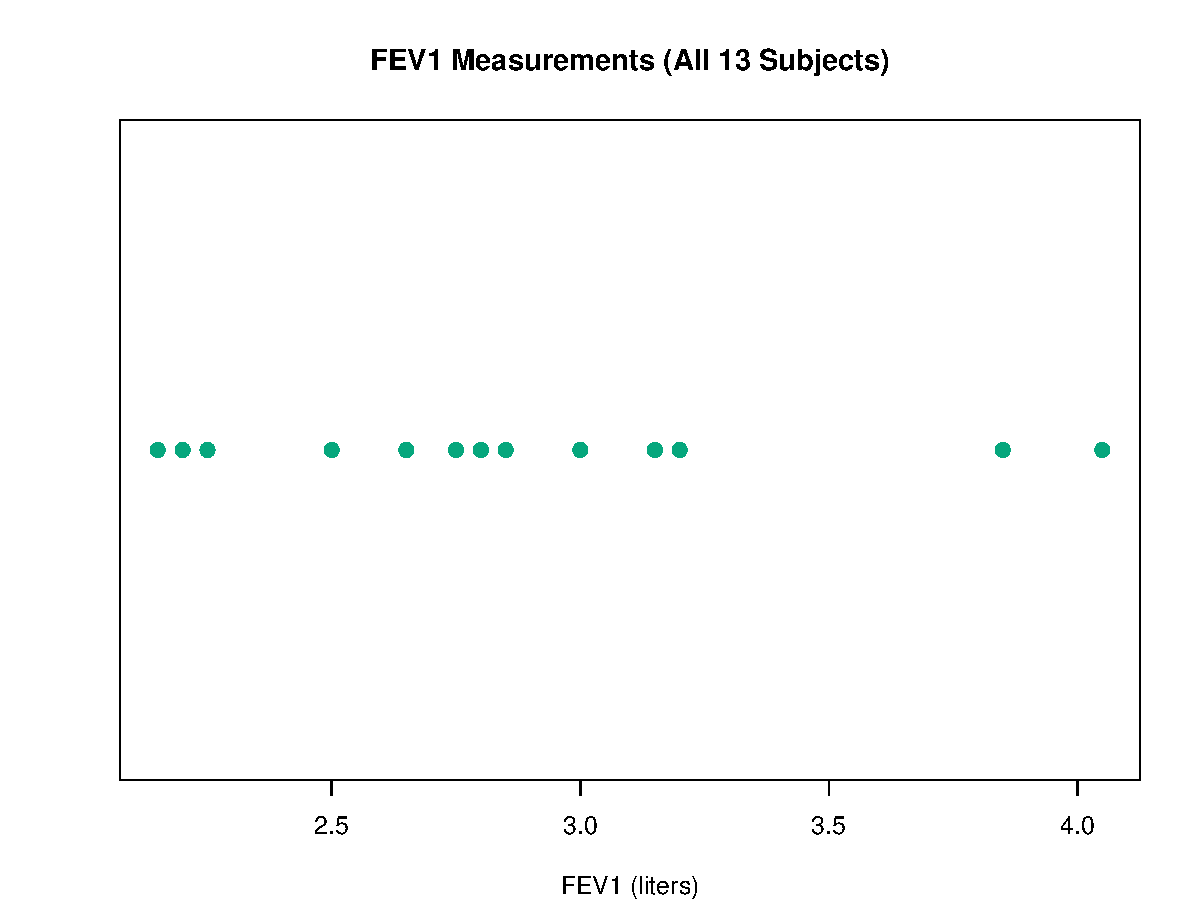
\includegraphics[width=0.7\textwidth]{../code/dotplot_fev1.pdf}
\caption{Example dot plot showing individual FEV1 measurements}
\end{figure}

\textbf{Assignment Tasks:}

\begin{enumerate}
\item Calculate descriptive statistics (mean, median, SD, range) for FEV1 by gender
\item Create comprehensive visualizations including:
   \begin{itemize}
   \item Geographic map showing state-level respiratory disease rates
   \item Multi-panel plot combining histogram, box plot, and dot plot
   \item BMI-FEV1 correlation analysis with trend lines
   \item Risk factor visualization (smoking, age, gender effects)
   \end{itemize}
\item Apply advanced analysis approaches:
   \begin{itemize}
   \item Risk ratio calculations where appropriate
   \item Correlation testing between variables
   \item Age-adjustment techniques for rate comparisons
   \item Professional publication-ready plot formatting
   \end{itemize}
\end{enumerate}

\subsection{Deliverables}

Submit the following files via Canvas:

\begin{enumerate}
\item \texttt{week1\_lab\_[lastname].R} - R script with all exercises
\item \texttt{week1\_lab\_report\_[lastname].pdf} - Brief report (1-2 pages) including:
   \begin{itemize}
   \item Summary statistics tables
   \item Key visualizations
   \item Brief interpretation of FEV1 findings
   \end{itemize}
\end{enumerate}

\section{Additional Resources}

\begin{itemize}
\item \textbf{R Documentation:} \url{https://www.rdocumentation.org/}
\item \textbf{RStudio Cheatsheets:} \url{https://posit.co/resources/cheatsheets/}
\item \textbf{Biostatistics with R:} \url{https://cran.r-project.org/web/views/MedicalImaging.html}
\end{itemize}

\end{document}